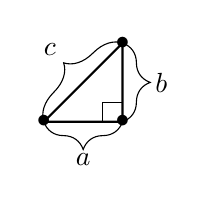
\begin{tikzpicture}
  \def\trilen{1}
  \def\triht{1}
  \coordinate (A) at (0,0);
  \coordinate (B) at (\trilen,0);
  \coordinate (C) at (\trilen,\triht);

  \def\squareside{.25}
  \draw (B) -- (\trilen,\squareside) -- (\trilen-\squareside,\squareside) -- (\trilen-\squareside,0);

  \draw[thick] node {$\bullet$} (A)
  -- (B) node {$\bullet$}
  -- (C) node {$\bullet$}
  -- (A);
  \draw [decorate,decoration={brace,amplitude=10pt,mirror},xshift=-4pt,yshift=0pt] (A) -- (B) node [midway,below,yshift=-8pt] {$a$};
  \draw [decorate,decoration={brace,amplitude=10pt,mirror},xshift=-4pt,yshift=0pt] (B) -- (C) node [midway,xshift=14pt] {$b$};
  \draw [decorate,decoration={brace,amplitude=10pt,mirror},xshift=-4pt,yshift=0pt] (C) -- (A) node [midway,xshift=-12pt,yshift=12pt] {$c$};
\end{tikzpicture}
